% Created by tikzDevice version 0.12.3 on 2020-01-08 13:37:48
% !TEX encoding = UTF-8 Unicode
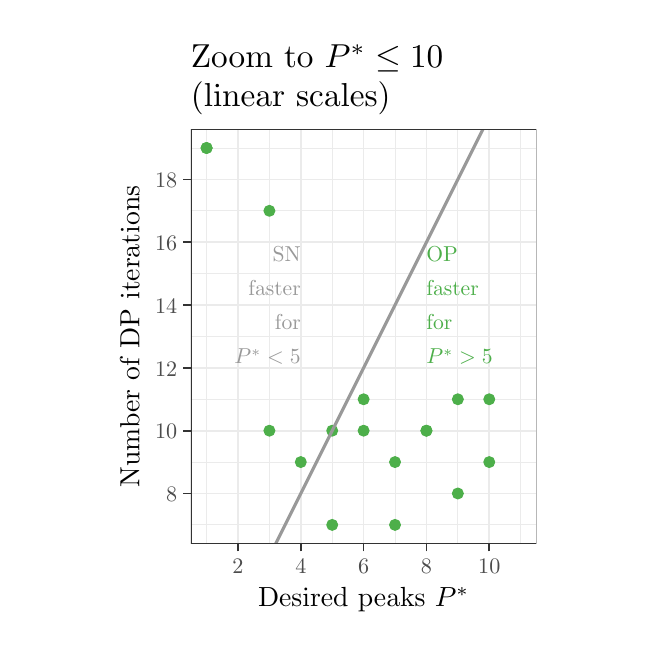
\begin{tikzpicture}[x=1pt,y=1pt]
\definecolor{fillColor}{RGB}{255,255,255}
\path[use as bounding box,fill=fillColor,fill opacity=0.00] (0,0) rectangle (216.81,216.81);
\begin{scope}
\path[clip] ( 27.50,  0.00) rectangle (189.31,216.81);
\definecolor{drawColor}{RGB}{255,255,255}
\definecolor{fillColor}{RGB}{255,255,255}

\path[draw=drawColor,line width= 0.6pt,line join=round,line cap=round,fill=fillColor] ( 27.50,  0.00) rectangle (189.31,216.81);
\end{scope}
\begin{scope}
\path[clip] ( 58.97, 30.33) rectangle (183.81,180.14);
\definecolor{fillColor}{RGB}{255,255,255}

\path[fill=fillColor] ( 58.97, 30.33) rectangle (183.81,180.14);
\definecolor{drawColor}{gray}{0.92}

\path[draw=drawColor,line width= 0.3pt,line join=round] ( 58.97, 37.14) --
	(183.81, 37.14);

\path[draw=drawColor,line width= 0.3pt,line join=round] ( 58.97, 59.84) --
	(183.81, 59.84);

\path[draw=drawColor,line width= 0.3pt,line join=round] ( 58.97, 82.53) --
	(183.81, 82.53);

\path[draw=drawColor,line width= 0.3pt,line join=round] ( 58.97,105.23) --
	(183.81,105.23);

\path[draw=drawColor,line width= 0.3pt,line join=round] ( 58.97,127.93) --
	(183.81,127.93);

\path[draw=drawColor,line width= 0.3pt,line join=round] ( 58.97,150.63) --
	(183.81,150.63);

\path[draw=drawColor,line width= 0.3pt,line join=round] ( 58.97,173.33) --
	(183.81,173.33);

\path[draw=drawColor,line width= 0.3pt,line join=round] ( 64.65, 30.33) --
	( 64.65,180.14);

\path[draw=drawColor,line width= 0.3pt,line join=round] ( 87.35, 30.33) --
	( 87.35,180.14);

\path[draw=drawColor,line width= 0.3pt,line join=round] (110.04, 30.33) --
	(110.04,180.14);

\path[draw=drawColor,line width= 0.3pt,line join=round] (132.74, 30.33) --
	(132.74,180.14);

\path[draw=drawColor,line width= 0.3pt,line join=round] (155.44, 30.33) --
	(155.44,180.14);

\path[draw=drawColor,line width= 0.3pt,line join=round] (178.14, 30.33) --
	(178.14,180.14);

\path[draw=drawColor,line width= 0.6pt,line join=round] ( 58.97, 48.49) --
	(183.81, 48.49);

\path[draw=drawColor,line width= 0.6pt,line join=round] ( 58.97, 71.18) --
	(183.81, 71.18);

\path[draw=drawColor,line width= 0.6pt,line join=round] ( 58.97, 93.88) --
	(183.81, 93.88);

\path[draw=drawColor,line width= 0.6pt,line join=round] ( 58.97,116.58) --
	(183.81,116.58);

\path[draw=drawColor,line width= 0.6pt,line join=round] ( 58.97,139.28) --
	(183.81,139.28);

\path[draw=drawColor,line width= 0.6pt,line join=round] ( 58.97,161.98) --
	(183.81,161.98);

\path[draw=drawColor,line width= 0.6pt,line join=round] ( 76.00, 30.33) --
	( 76.00,180.14);

\path[draw=drawColor,line width= 0.6pt,line join=round] ( 98.69, 30.33) --
	( 98.69,180.14);

\path[draw=drawColor,line width= 0.6pt,line join=round] (121.39, 30.33) --
	(121.39,180.14);

\path[draw=drawColor,line width= 0.6pt,line join=round] (144.09, 30.33) --
	(144.09,180.14);

\path[draw=drawColor,line width= 0.6pt,line join=round] (166.79, 30.33) --
	(166.79,180.14);
\definecolor{drawColor}{RGB}{77,175,74}
\definecolor{fillColor}{RGB}{77,175,74}

\path[draw=drawColor,line width= 0.4pt,line join=round,line cap=round,fill=fillColor] ( 64.65,173.33) circle (  1.96);

\path[draw=drawColor,line width= 0.4pt,line join=round,line cap=round,fill=fillColor] ( 87.35, 71.18) circle (  1.96);

\path[draw=drawColor,line width= 0.4pt,line join=round,line cap=round,fill=fillColor] ( 98.69, 59.84) circle (  1.96);

\path[draw=drawColor,line width= 0.4pt,line join=round,line cap=round,fill=fillColor] (110.04, 71.18) circle (  1.96);

\path[draw=drawColor,line width= 0.4pt,line join=round,line cap=round,fill=fillColor] (121.39, 82.53) circle (  1.96);

\path[draw=drawColor,line width= 0.4pt,line join=round,line cap=round,fill=fillColor] (132.74, 37.14) circle (  1.96);

\path[draw=drawColor,line width= 0.4pt,line join=round,line cap=round,fill=fillColor] (144.09, 71.18) circle (  1.96);

\path[draw=drawColor,line width= 0.4pt,line join=round,line cap=round,fill=fillColor] (155.44, 82.53) circle (  1.96);

\path[draw=drawColor,line width= 0.4pt,line join=round,line cap=round,fill=fillColor] (166.79, 59.84) circle (  1.96);

\path[draw=drawColor,line width= 0.4pt,line join=round,line cap=round,fill=fillColor] ( 64.65,173.33) circle (  1.96);

\path[draw=drawColor,line width= 0.4pt,line join=round,line cap=round,fill=fillColor] ( 87.35,150.63) circle (  1.96);

\path[draw=drawColor,line width= 0.4pt,line join=round,line cap=round,fill=fillColor] (110.04, 37.14) circle (  1.96);

\path[draw=drawColor,line width= 0.4pt,line join=round,line cap=round,fill=fillColor] (121.39, 71.18) circle (  1.96);

\path[draw=drawColor,line width= 0.4pt,line join=round,line cap=round,fill=fillColor] (132.74, 59.84) circle (  1.96);

\path[draw=drawColor,line width= 0.4pt,line join=round,line cap=round,fill=fillColor] (144.09, 71.18) circle (  1.96);

\path[draw=drawColor,line width= 0.4pt,line join=round,line cap=round,fill=fillColor] (155.44, 48.49) circle (  1.96);

\path[draw=drawColor,line width= 0.4pt,line join=round,line cap=round,fill=fillColor] (166.79, 82.53) circle (  1.96);
\definecolor{drawColor}{gray}{0.60}

\path[draw=drawColor,line width= 1.1pt,line join=round] ( 74.45,  0.00) -- (182.86,216.81);

\node[text=drawColor,anchor=base east,inner sep=0pt, outer sep=0pt, scale=  0.78] at ( 98.69,132.15) {SN};

\node[text=drawColor,anchor=base east,inner sep=0pt, outer sep=0pt, scale=  0.78] at ( 98.69,119.86) {faster};

\node[text=drawColor,anchor=base east,inner sep=0pt, outer sep=0pt, scale=  0.78] at ( 98.69,107.57) {for};

\node[text=drawColor,anchor=base east,inner sep=0pt, outer sep=0pt, scale=  0.78] at ( 98.69, 95.28) {$P^*<5$};
\definecolor{drawColor}{RGB}{77,175,74}

\node[text=drawColor,anchor=base west,inner sep=0pt, outer sep=0pt, scale=  0.78] at (144.09,132.15) {OP};

\node[text=drawColor,anchor=base west,inner sep=0pt, outer sep=0pt, scale=  0.78] at (144.09,119.86) {faster};

\node[text=drawColor,anchor=base west,inner sep=0pt, outer sep=0pt, scale=  0.78] at (144.09,107.57) {for};

\node[text=drawColor,anchor=base west,inner sep=0pt, outer sep=0pt, scale=  0.78] at (144.09, 95.28) {$P^*>5$};
\definecolor{drawColor}{gray}{0.20}

\path[draw=drawColor,line width= 0.6pt,line join=round,line cap=round] ( 58.97, 30.33) rectangle (183.81,180.14);
\end{scope}
\begin{scope}
\path[clip] (  0.00,  0.00) rectangle (216.81,216.81);
\definecolor{drawColor}{gray}{0.30}

\node[text=drawColor,anchor=base east,inner sep=0pt, outer sep=0pt, scale=  0.80] at ( 54.02, 45.53) {8};

\node[text=drawColor,anchor=base east,inner sep=0pt, outer sep=0pt, scale=  0.80] at ( 54.02, 68.23) {10};

\node[text=drawColor,anchor=base east,inner sep=0pt, outer sep=0pt, scale=  0.80] at ( 54.02, 90.93) {12};

\node[text=drawColor,anchor=base east,inner sep=0pt, outer sep=0pt, scale=  0.80] at ( 54.02,113.62) {14};

\node[text=drawColor,anchor=base east,inner sep=0pt, outer sep=0pt, scale=  0.80] at ( 54.02,136.32) {16};

\node[text=drawColor,anchor=base east,inner sep=0pt, outer sep=0pt, scale=  0.80] at ( 54.02,159.02) {18};
\end{scope}
\begin{scope}
\path[clip] (  0.00,  0.00) rectangle (216.81,216.81);
\definecolor{drawColor}{gray}{0.20}

\path[draw=drawColor,line width= 0.6pt,line join=round] ( 56.22, 48.49) --
	( 58.97, 48.49);

\path[draw=drawColor,line width= 0.6pt,line join=round] ( 56.22, 71.18) --
	( 58.97, 71.18);

\path[draw=drawColor,line width= 0.6pt,line join=round] ( 56.22, 93.88) --
	( 58.97, 93.88);

\path[draw=drawColor,line width= 0.6pt,line join=round] ( 56.22,116.58) --
	( 58.97,116.58);

\path[draw=drawColor,line width= 0.6pt,line join=round] ( 56.22,139.28) --
	( 58.97,139.28);

\path[draw=drawColor,line width= 0.6pt,line join=round] ( 56.22,161.98) --
	( 58.97,161.98);
\end{scope}
\begin{scope}
\path[clip] (  0.00,  0.00) rectangle (216.81,216.81);
\definecolor{drawColor}{gray}{0.20}

\path[draw=drawColor,line width= 0.6pt,line join=round] ( 76.00, 27.58) --
	( 76.00, 30.33);

\path[draw=drawColor,line width= 0.6pt,line join=round] ( 98.69, 27.58) --
	( 98.69, 30.33);

\path[draw=drawColor,line width= 0.6pt,line join=round] (121.39, 27.58) --
	(121.39, 30.33);

\path[draw=drawColor,line width= 0.6pt,line join=round] (144.09, 27.58) --
	(144.09, 30.33);

\path[draw=drawColor,line width= 0.6pt,line join=round] (166.79, 27.58) --
	(166.79, 30.33);
\end{scope}
\begin{scope}
\path[clip] (  0.00,  0.00) rectangle (216.81,216.81);
\definecolor{drawColor}{gray}{0.30}

\node[text=drawColor,anchor=base,inner sep=0pt, outer sep=0pt, scale=  0.80] at ( 76.00, 19.46) {2};

\node[text=drawColor,anchor=base,inner sep=0pt, outer sep=0pt, scale=  0.80] at ( 98.69, 19.46) {4};

\node[text=drawColor,anchor=base,inner sep=0pt, outer sep=0pt, scale=  0.80] at (121.39, 19.46) {6};

\node[text=drawColor,anchor=base,inner sep=0pt, outer sep=0pt, scale=  0.80] at (144.09, 19.46) {8};

\node[text=drawColor,anchor=base,inner sep=0pt, outer sep=0pt, scale=  0.80] at (166.79, 19.46) {10};
\end{scope}
\begin{scope}
\path[clip] (  0.00,  0.00) rectangle (216.81,216.81);
\definecolor{drawColor}{RGB}{0,0,0}

\node[text=drawColor,anchor=base,inner sep=0pt, outer sep=0pt, scale=  1.00] at (121.39,  7.62) {Desired peaks $P^*$};
\end{scope}
\begin{scope}
\path[clip] (  0.00,  0.00) rectangle (216.81,216.81);
\definecolor{drawColor}{RGB}{0,0,0}

\node[text=drawColor,rotate= 90.00,anchor=base,inner sep=0pt, outer sep=0pt, scale=  1.00] at ( 40.39,105.23) {Number of DP iterations};
\end{scope}
\begin{scope}
\path[clip] (  0.00,  0.00) rectangle (216.81,216.81);
\definecolor{drawColor}{RGB}{0,0,0}

\node[text=drawColor,anchor=base west,inner sep=0pt, outer sep=0pt, scale=  1.20] at ( 58.97,202.44) {Zoom to $P^* \leq 10$};

\node[text=drawColor,anchor=base west,inner sep=0pt, outer sep=0pt, scale=  1.20] at ( 58.97,188.18) {(linear scales)};
\end{scope}
\end{tikzpicture}
